\chapter{原型系统设计与实现}
本文的第三章和第四章提出了基于深度学习的毫米波雷达目标点检测方案和毫米波雷达点云配准方案。本章将介绍如何将这两种方案结合起来,构建一个完整的毫米波雷达点云配准原型系统,并将该系统接入到本课题组研发的校园安防系统中,用于多毫米波雷达场景的毫米波雷达点云数据融合,并且用融合后的数据进行目标检测和跟踪。本章将从系统整体设计、系统实现、系统测试三个方面介绍原型系统的设计和实现。
\section{系统设计}
\subsection{系统架构}
基于本文第三章和第四章提出的毫米波雷达目标点检测方案和毫米波雷达点云配准方案,本文将设计一个完整的毫米波雷达点云配准原型系统。系统的整体架构如图\ref{fig:系统架构}所示。
\begin{figure}[htbp]
    \centering
    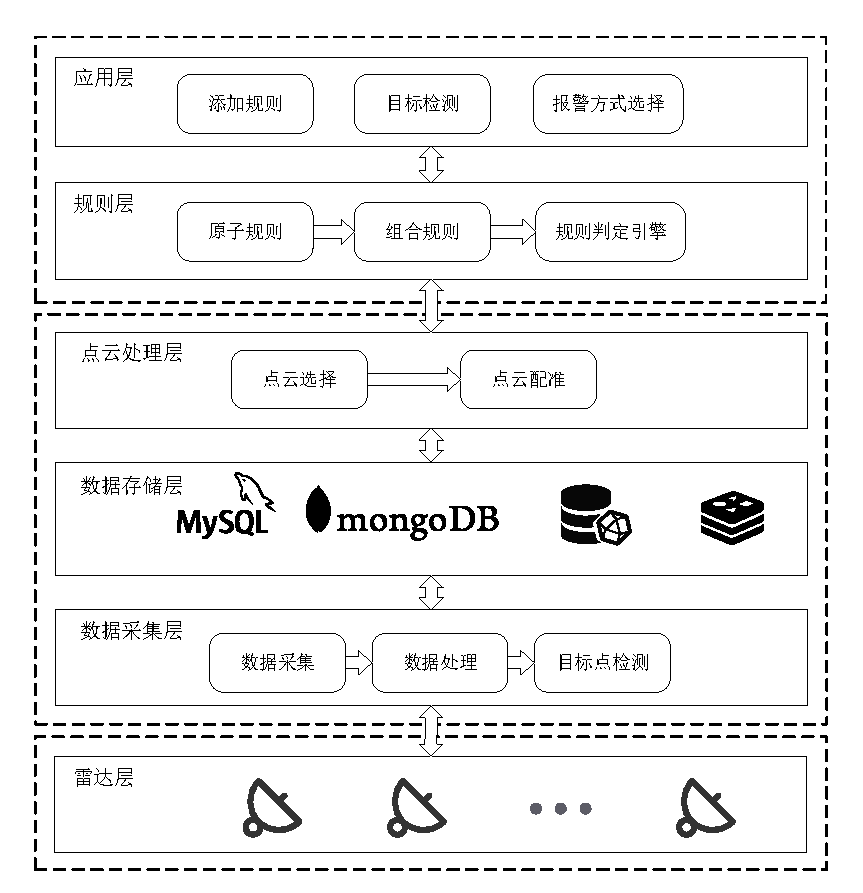
\includegraphics[width=0.9\linewidth]{figures/系统架构.pdf}
    \caption{系统架构}
    \label{fig:系统架构}
\end{figure}
\par
本系统主要分为雷达层、数据采集层,数据存储层、点云处理层、规则层和应用层。雷达层由多个IWR6843毫米波雷达组成,负责环境检测并将回波信号转换为二进制数据传输给数据采集层。数据采集层主要负责接收雷达层传来的二进制数据,将二进制数据转换为点云数据,然后将点云数据存储到数据存储层。数据存储层主要负责存储数据采集层传来的点云数据和规则层设置的规则参数。点云处理层主要负责接收数据存储层传来的点云数据,然后对点云数据进行处理,包括点云的预处理、待配准点云的选择、点云的配准。规则层主要负责接收点云处理层传来的配准后的点云数据,根据预先设定的规则判断点云数据是否满足规则,如果满足规则将触发的规则传给应用层。应用层主要负责接收规则层传来的触发的规则,根据触发的规则进行相应的处理,包括将点云数据传给目标检测和跟踪模块,将点云数据传给数据融合模块等。
\subsection{系统详细设计}

\par
(1)雷达层
\par
雷达层由多个IWR6843毫米波雷达组成,负责环境检测并将回波信号转换为二进制数据传输给数据采集层。IWR6843毫米波雷达是德州仪器公司推出的一款毫米波雷达,工作频率为60GHz,具有高分辨率、高精度、高灵敏度等特点。IWR6843毫米波雷达可以通过SPI接口将回波信号转换为二进制数据传输给数据采集层。

\par
(2)数据采集层
\par
数据采集层负责接收雷达层传来的二进制数据,由数据采集模块、数据处理模块和目标点检测模块组成。数据采集模块负责接收雷达层传来的实时二进制数据。为了保证目标检测的实时性以及系统的健壮性,在数据采集模块以及数据处理模块之间使用消息队列进行解耦,通过异步处理的方式进行削峰填谷提升歘同的吞吐量,根据雷达设备的ID,作为消息队列的topic,将数据采集模块采集到的数据发送到消息队列中过程如图\ref{fig:数据采集模块}所示。数据处理模块负责接收数据采集模块传来的二进制数据,然后对二进制数据进行处理,将二进制数据转换为点云数据。目标点检测模块负责接收数据处理模块传来的点云数据,然后对点云数据进行目标点检测。数据采集层的处理过程如图\ref{fig:采集模块处理过程}所示。
\begin{figure}[htbp]
    \centering
    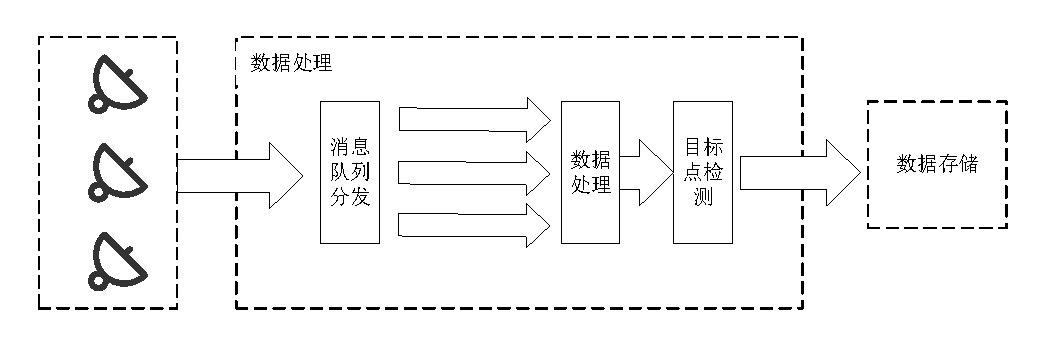
\includegraphics[width=0.9\linewidth]{figures/数据采集模块.pdf}
    \caption{数据采集模块}
    \label{fig:数据采集模块}
\end{figure}

\begin{figure}[htbp]
    \centering
    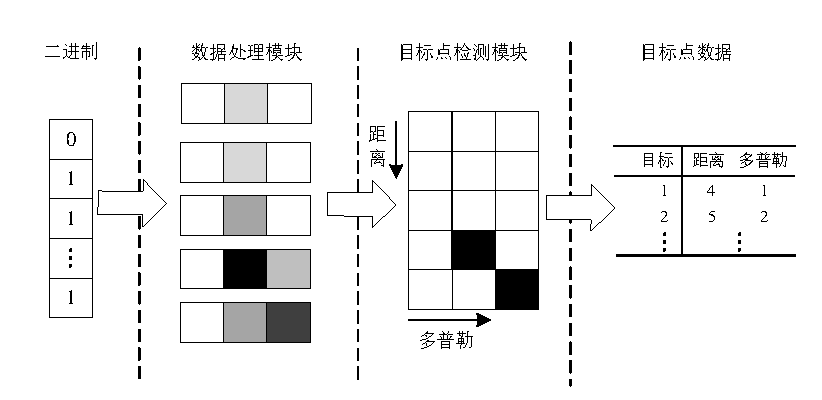
\includegraphics[width=0.9\linewidth]{figures/采集模块处理过程.pdf}
    \caption{采集模块处理过程}
    \label{fig:采集模块处理过程}
\end{figure}

\par
(3)数据存储层
\par
数据存储层主要负责存储数据采集层传来的点云数据,主要由MySQL、MongoDB、Redis、HDFS等数据库组成,负责存储点云数据。MongoDB负责存储点云数据的原始数据;MySQL负责存储经过目标点检测的点云数据和经过点云配准的点云数据;Redis负责储存上层规则的缓存;HDFS负责存储预训练的目标点检测模型和配准模型。

\par
(4)点云处理层
\par
点云处理层主要负责接收数据存储层传来的点云数据,然后对点云数据进行处理,点云处理层主要由点云选择模块、点云配准模块组成。点云选择模块负责选择待配准的点云数据,包括选择待配准的点云数据的时间、选择待配准的点云数据的空间等;点云配准模块负责对待配准的点云数据进行配准,包括点云的特征提取、点云的特征匹配、点云的配准等,如图\ref{fig:点云处理层}所示。

\begin{figure}[htbp]
    \centering
    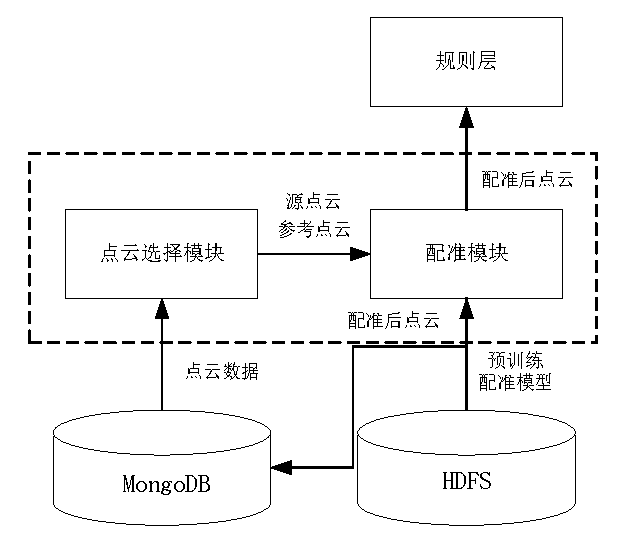
\includegraphics[width=0.6\linewidth]{figures/点云处理层.pdf}
    \caption{点云处理层}
    \label{fig:点云处理层}
\end{figure}

\par
(5)规则层
\par
规则层主要负责接收点云处理层传来的配准后的点云数据,然后根据预先设定的规则判断点云数据是否满足规则,如果满足规则将触发的规则传给应用层。规则层主要由原子规则模块、组合规则模块、规则引擎模块组成。原子规则模块负责定义原子规则;组合规则模块负责定义组合规则,对规则进行交集或者并集的操作;规则引擎模块负责根据原子规则和组合规则判断点云数据是否满足规则,如图\ref{fig:规则层}所示。

\begin{figure}[htbp]
    \centering
    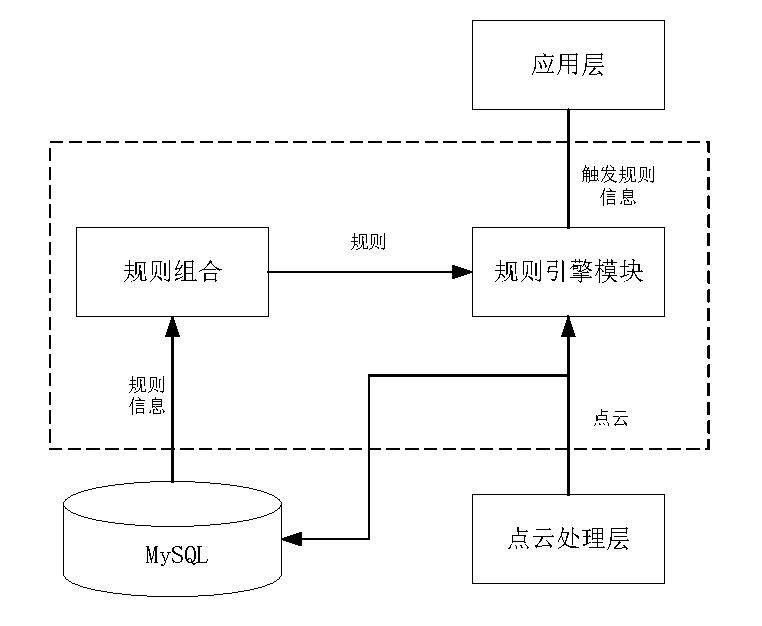
\includegraphics[width=0.6\linewidth]{figures/规则层.pdf}
    \caption{规则层}
    \label{fig:规则层}
\end{figure}

\par
(6)应用层
\par
应用层主要负责接收规则层传来的触发的规则,然后根据触发的规则进行相应的处理,包括将点云数据传给目标检测和跟踪模块,经检测到的目标轨迹传给可视化挂机模块等。应用层主要由目标检测和跟踪模块、可视化模块、报警模块组成。目标检测和跟踪模块负责接收点云数据,然后对点云数据进行目标检测和跟踪,最后将检测到的目标轨迹传给可视化模块;可视化模块负责接收目标检测和跟踪模块传来的目标轨迹,然后将目标轨迹可视化;报警模块负责接收规则层传来的触发的规则,然后根据触发的规则进行报警。
\section{系统测试}
\subsection{系统测试环境}
本节给出了原型系统部署的硬件环境和软件环境,如表\ref{硬件配置表}和表\ref{软件配置表}所示。
\par
(1)硬件环境
\par
\begin{table}[htbp]
	\centering
	\tabcolsep=3mm
	\caption{硬件配置表}
	\begin{tabular}{cccp{3cm}}
		\toprule
		设备 & 参数 &数量&用途 \\
		\midrule
		联想 ThinkStation P340 & \makecell[l]{内存:32G \\ 硬盘:2T \\ 显卡:GTX 1660 Super \\ CPU: Intel i7-11500} &1 & 部署校园安防系统以及点云检测和配准模块 \\
        IWR6843毫米波雷达 & \makecell[l]{发射天线:4 \\ 接收天线:3 \\ 开始频率:60.6GHz \\ 带宽: 2.249GHz} &3 & 环境感知 \\
        DCA1000 EVM & /  &3 & 采集数据 \\
		\bottomrule
	\end{tabular}
	\label{硬件配置表}
\end{table}

\par
(2)软件环境
使用Torch进行模型部署,MySQL存储包括规则信息、报警信息等业务信息,MongoDB负责存储点云数据的原始数据,JMETER进行大量雷达数据的压测。
\par
\begin{table}[htbp]
	\centering
	\tabcolsep=2cm
	\caption{软件配置表}
	\begin{tabular}{cc}
		\toprule
		软件 & 版本 \\
		\midrule
		Python & 3.10.13 \\
        Torch & 2.2.0  \\
        MySQL & 8.0.28 \\
        MongoDB & 5.0.5 \\
        Apache JMETER & 5.4.1 \\
		\bottomrule
	\end{tabular}
	\label{软件配置表}
\end{table}

\subsection{系统功能测试}
为了确保毫米波雷达点云配准原型系统的功能正常,本节进行了系统功能测试。系统功能测试主要包括点云数据采集功能测试、点云数据存储功能测试、点云数据处理功能测试、规则判断功能测试、目标检测和跟踪功能测试、可视化功能测试、报警功能测试等。本节将对与毫米波雷达点云检测与配准相关的功能,添加毫米波雷设备、点云数据采集、目标检测和跟踪功能的测试过程展开详细描述。完整系统功能测试的测试用例如表\ref{系统功能测试用例}所示。
\begin{table}
    \centering
    \tabcolsep=3mm
    \caption{系统功能测试用例}
    \begin{tabular}{ccp{3cm}c}
        \toprule
        测试用例编号 & 测试用例名称 & 预期结果 & 测试结果 \\
        \midrule
        0 & 添加雷达设备测试 & 雷达层能够在指定位置正确添加雷达设备& 通过 \\
        1 & 点云数据采集功能测试 & 数据采集模块能够正常接收雷达层传来的二进制数据 & 通过 \\
        2 & 点云数据存储功能测试 & 数据存储层能够正常存储数据采集层传来的点云数据 & 通过 \\
        3 & 点云数据处理功能测试 & 点云处理层能够正常接收数据存储层传来的点云数据 & 通过 \\
        4 & 规则判断功能测试 & 规则层能够正常判断点云数据是否满足规则 & 通过 \\
        5 & 目标检测和跟踪功能测试 & 目标检测和跟踪模块能够根据点云数据检测到目标并且跟踪目标轨迹 & 通过 \\
        6 & 可视化功能测试 & 可视化模块能够正常接收目标检测和跟踪模块传来的目标轨迹 & 通过 \\
        7 & 报警功能测试 & 报警模块能够正常接收规则层传来的触发的规则 & 通过 \\

        \bottomrule
    \end{tabular}
    \label{系统功能测试用例}
\end{table}

\par
(1)添加雷达设备测试
\par
添加雷达设备测试主要测试雷达层能否在指定位置正确添加雷达设备,使用指定的雷达SN号和雷达位置添加雷达设备,然后检查雷达设备是否添加成功。
\begin{figure}[htbp]
    \centering
    \subcaptionbox{添加雷达设备}{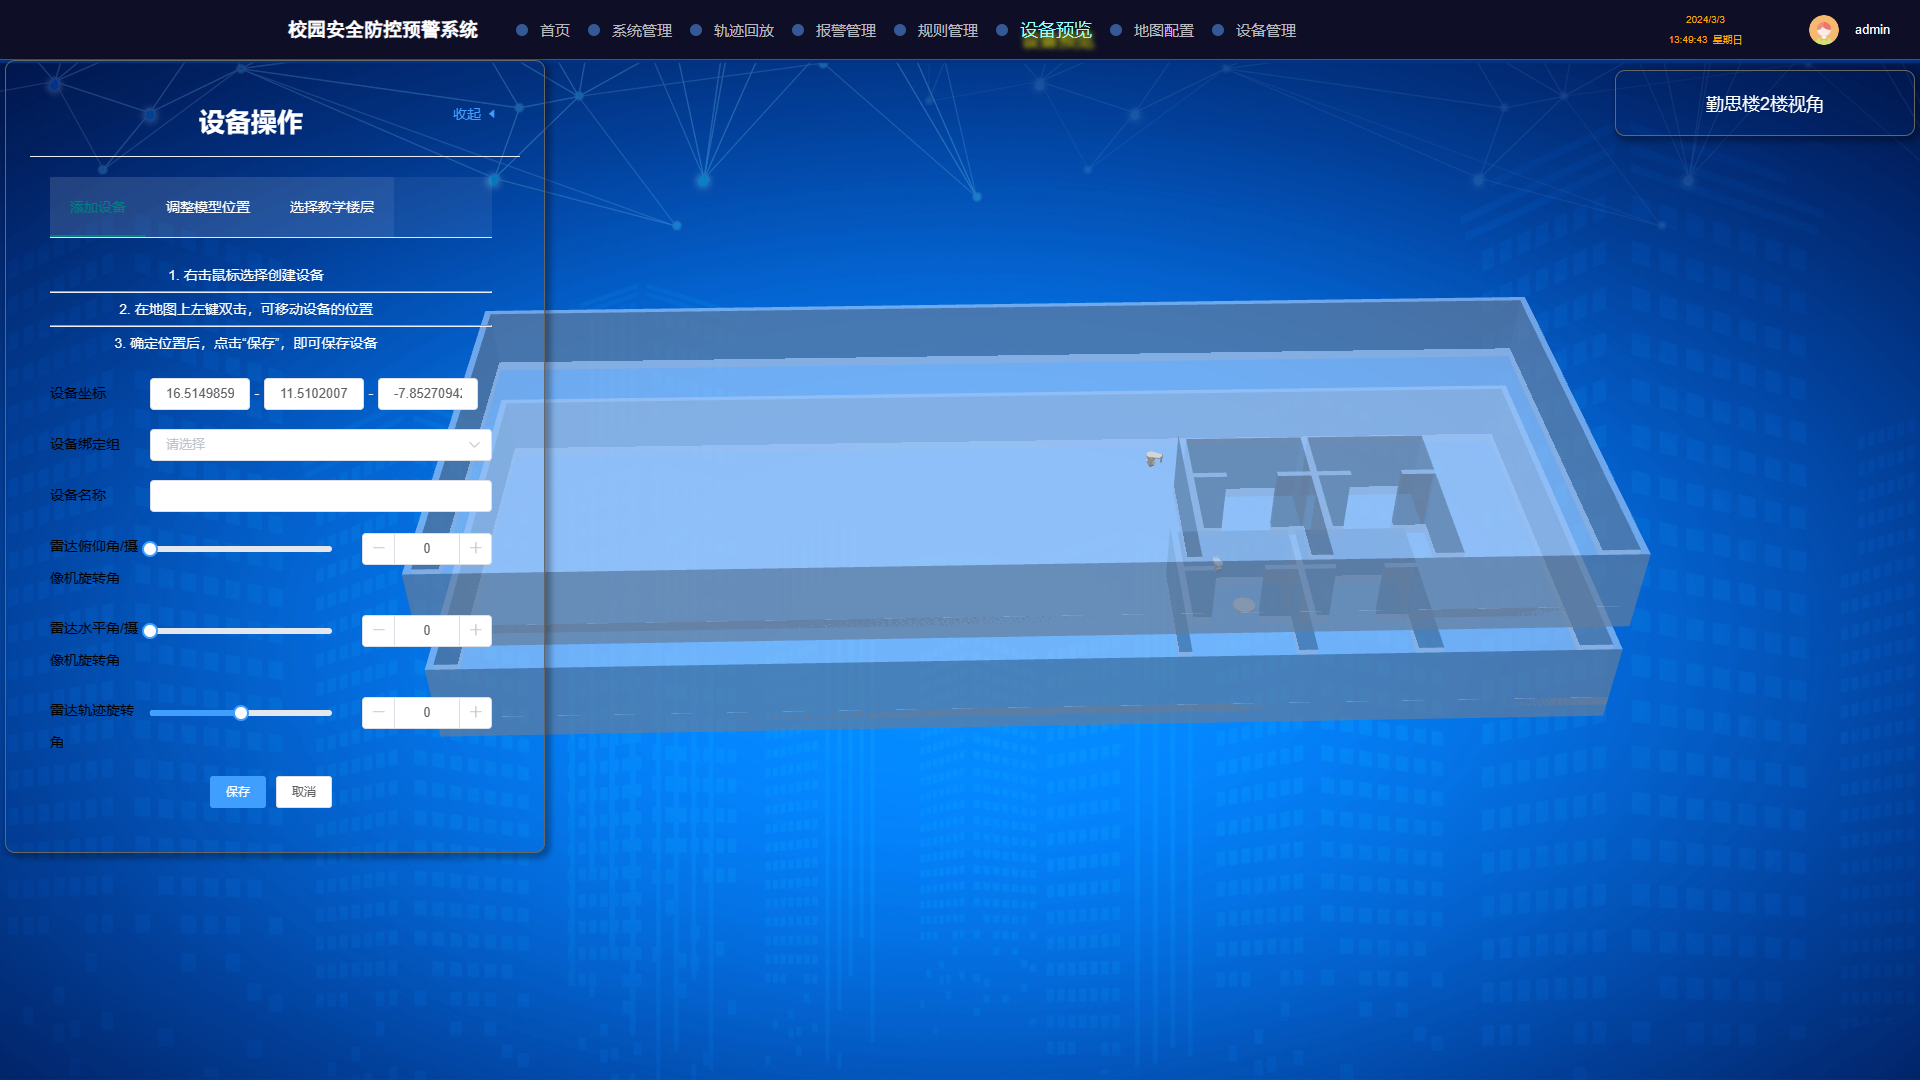
\includegraphics[width = 0.49\linewidth]{images/添加雷达设备.png}}
    \subcaptionbox{管理雷达设备}{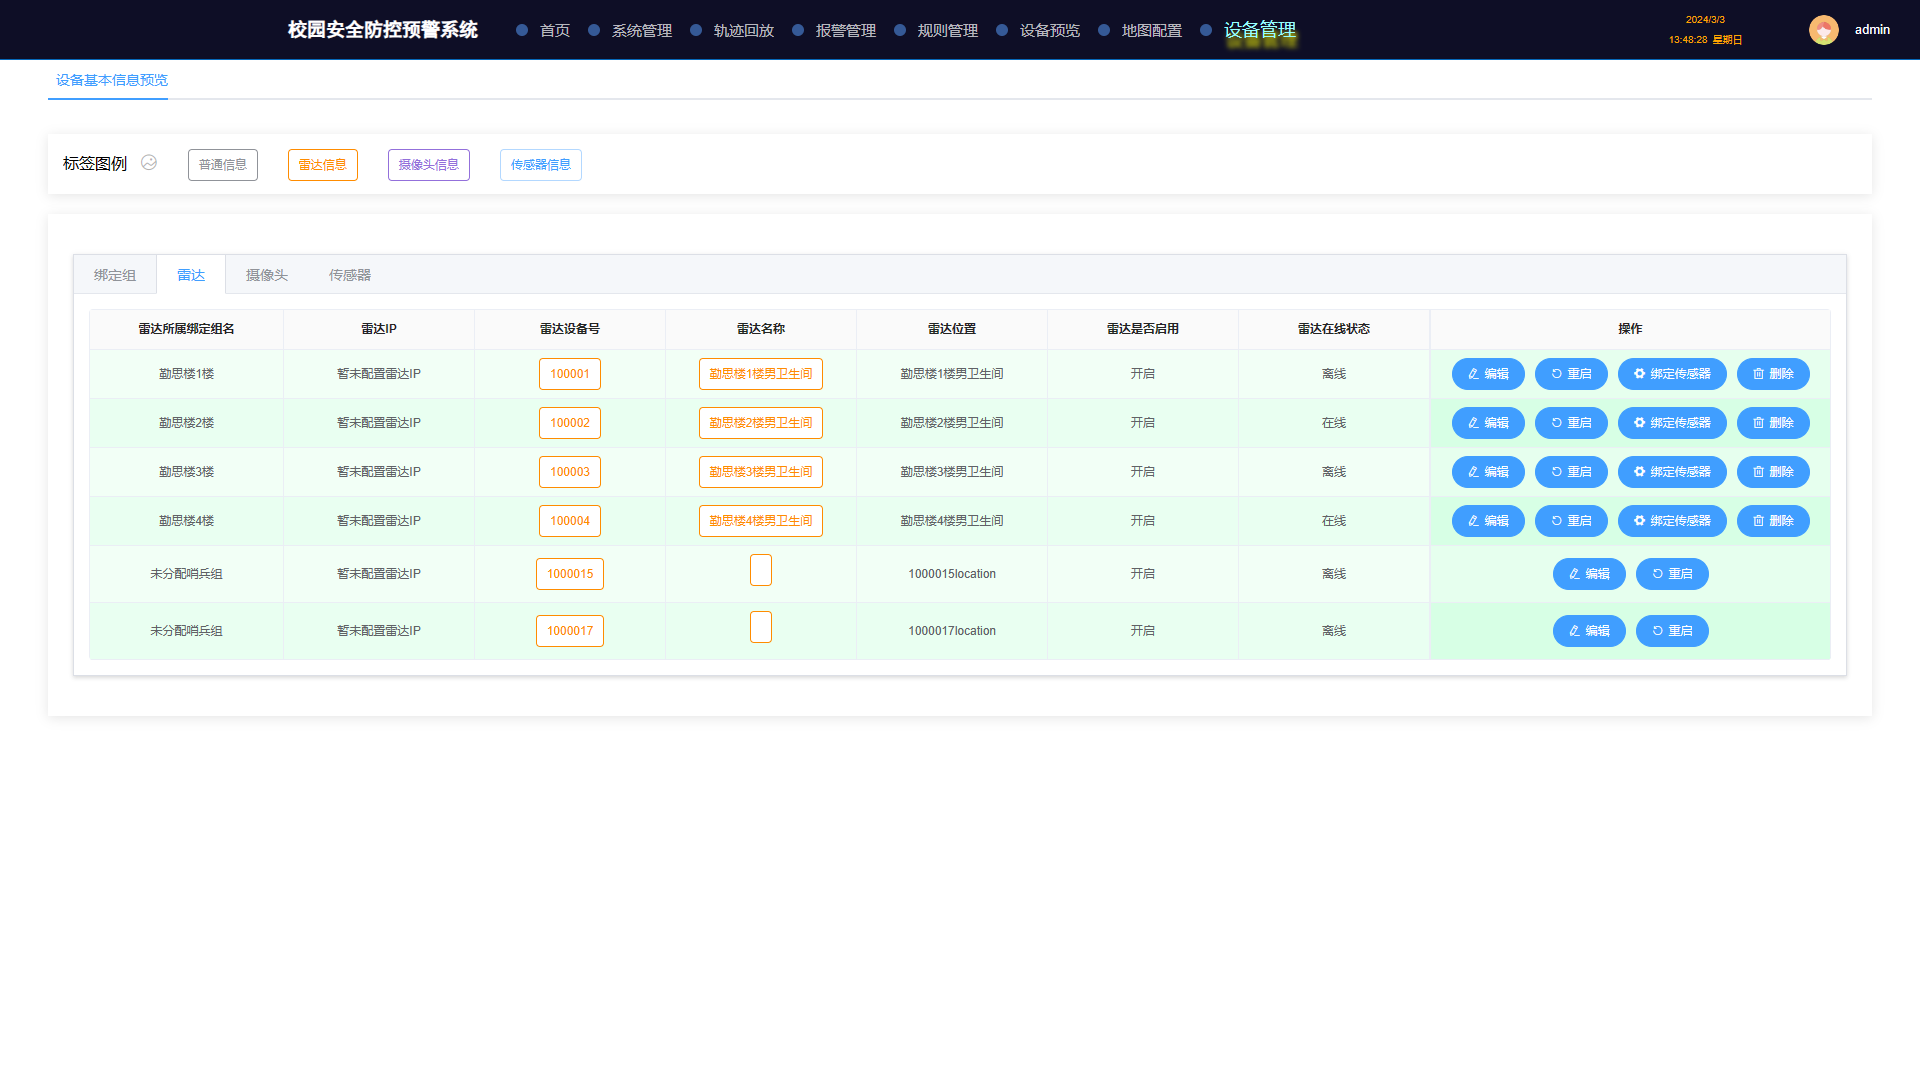
\includegraphics[width = 0.49\linewidth]{images/管理雷达设备.png}}
    \caption{添加雷达设备测试}
    \label{fig:添加雷达设备测试}    
\end{figure}
\par
(2)点云数据采集功能测试
\par
点云数据采集功能测试主要测试数据采集模块是否能够正常接收雷达层传来的二进制数据,数据处理模块是否能够正常接收数据采集模块传来的二进制数据,目标点检测模块是否能够正常接收数据处理模块传来的点云数据,点云数据采集模块过滤后的点云如图\ref{fig:点云数据采集功能测试}所示。
\begin{figure}[htbp]
    \centering
    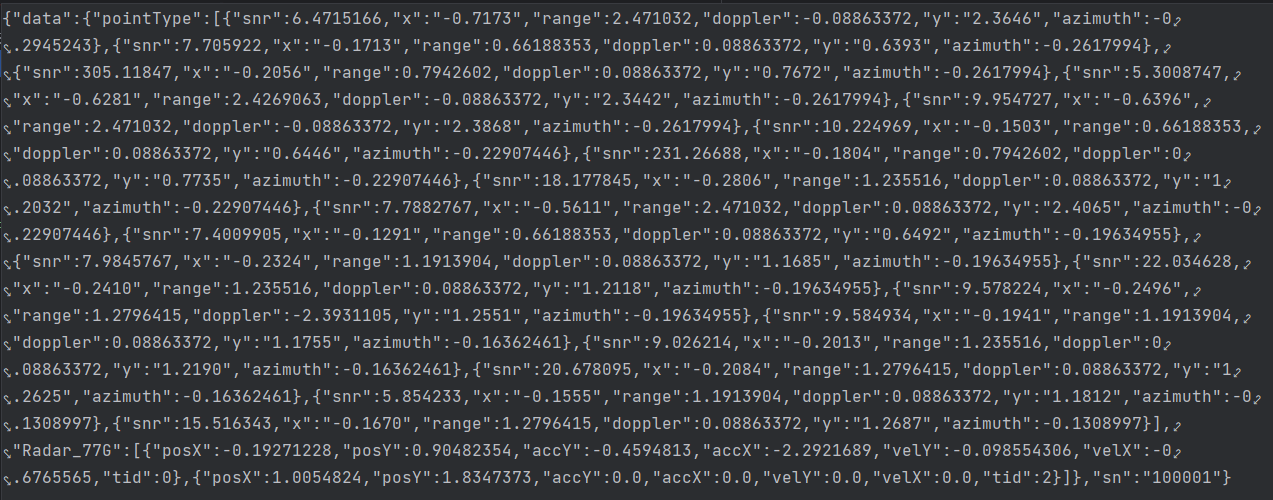
\includegraphics[width = 0.8\linewidth]{images/点云数据.png}
    \caption{点云数据采集功能测试}
    \label{fig:点云数据采集功能测试}    
\end{figure}

\par
(3)目标检测和跟踪功能测试
\par
收到点云数据后,目标检测模块根据点云数据检测到目标后,跟踪目标移动,使用目标移动的历史轨迹,绘制目标移动轨迹图,并将轨迹图传给可视化模块和存储模块。目标检测和目标轨迹绘制的效果分别如图\ref{目标检测}和\ref{目标历史轨迹}所示。

\begin{figure}[htbp]
    \centering
    \subcaptionbox{目标检测 \label{目标检测} }{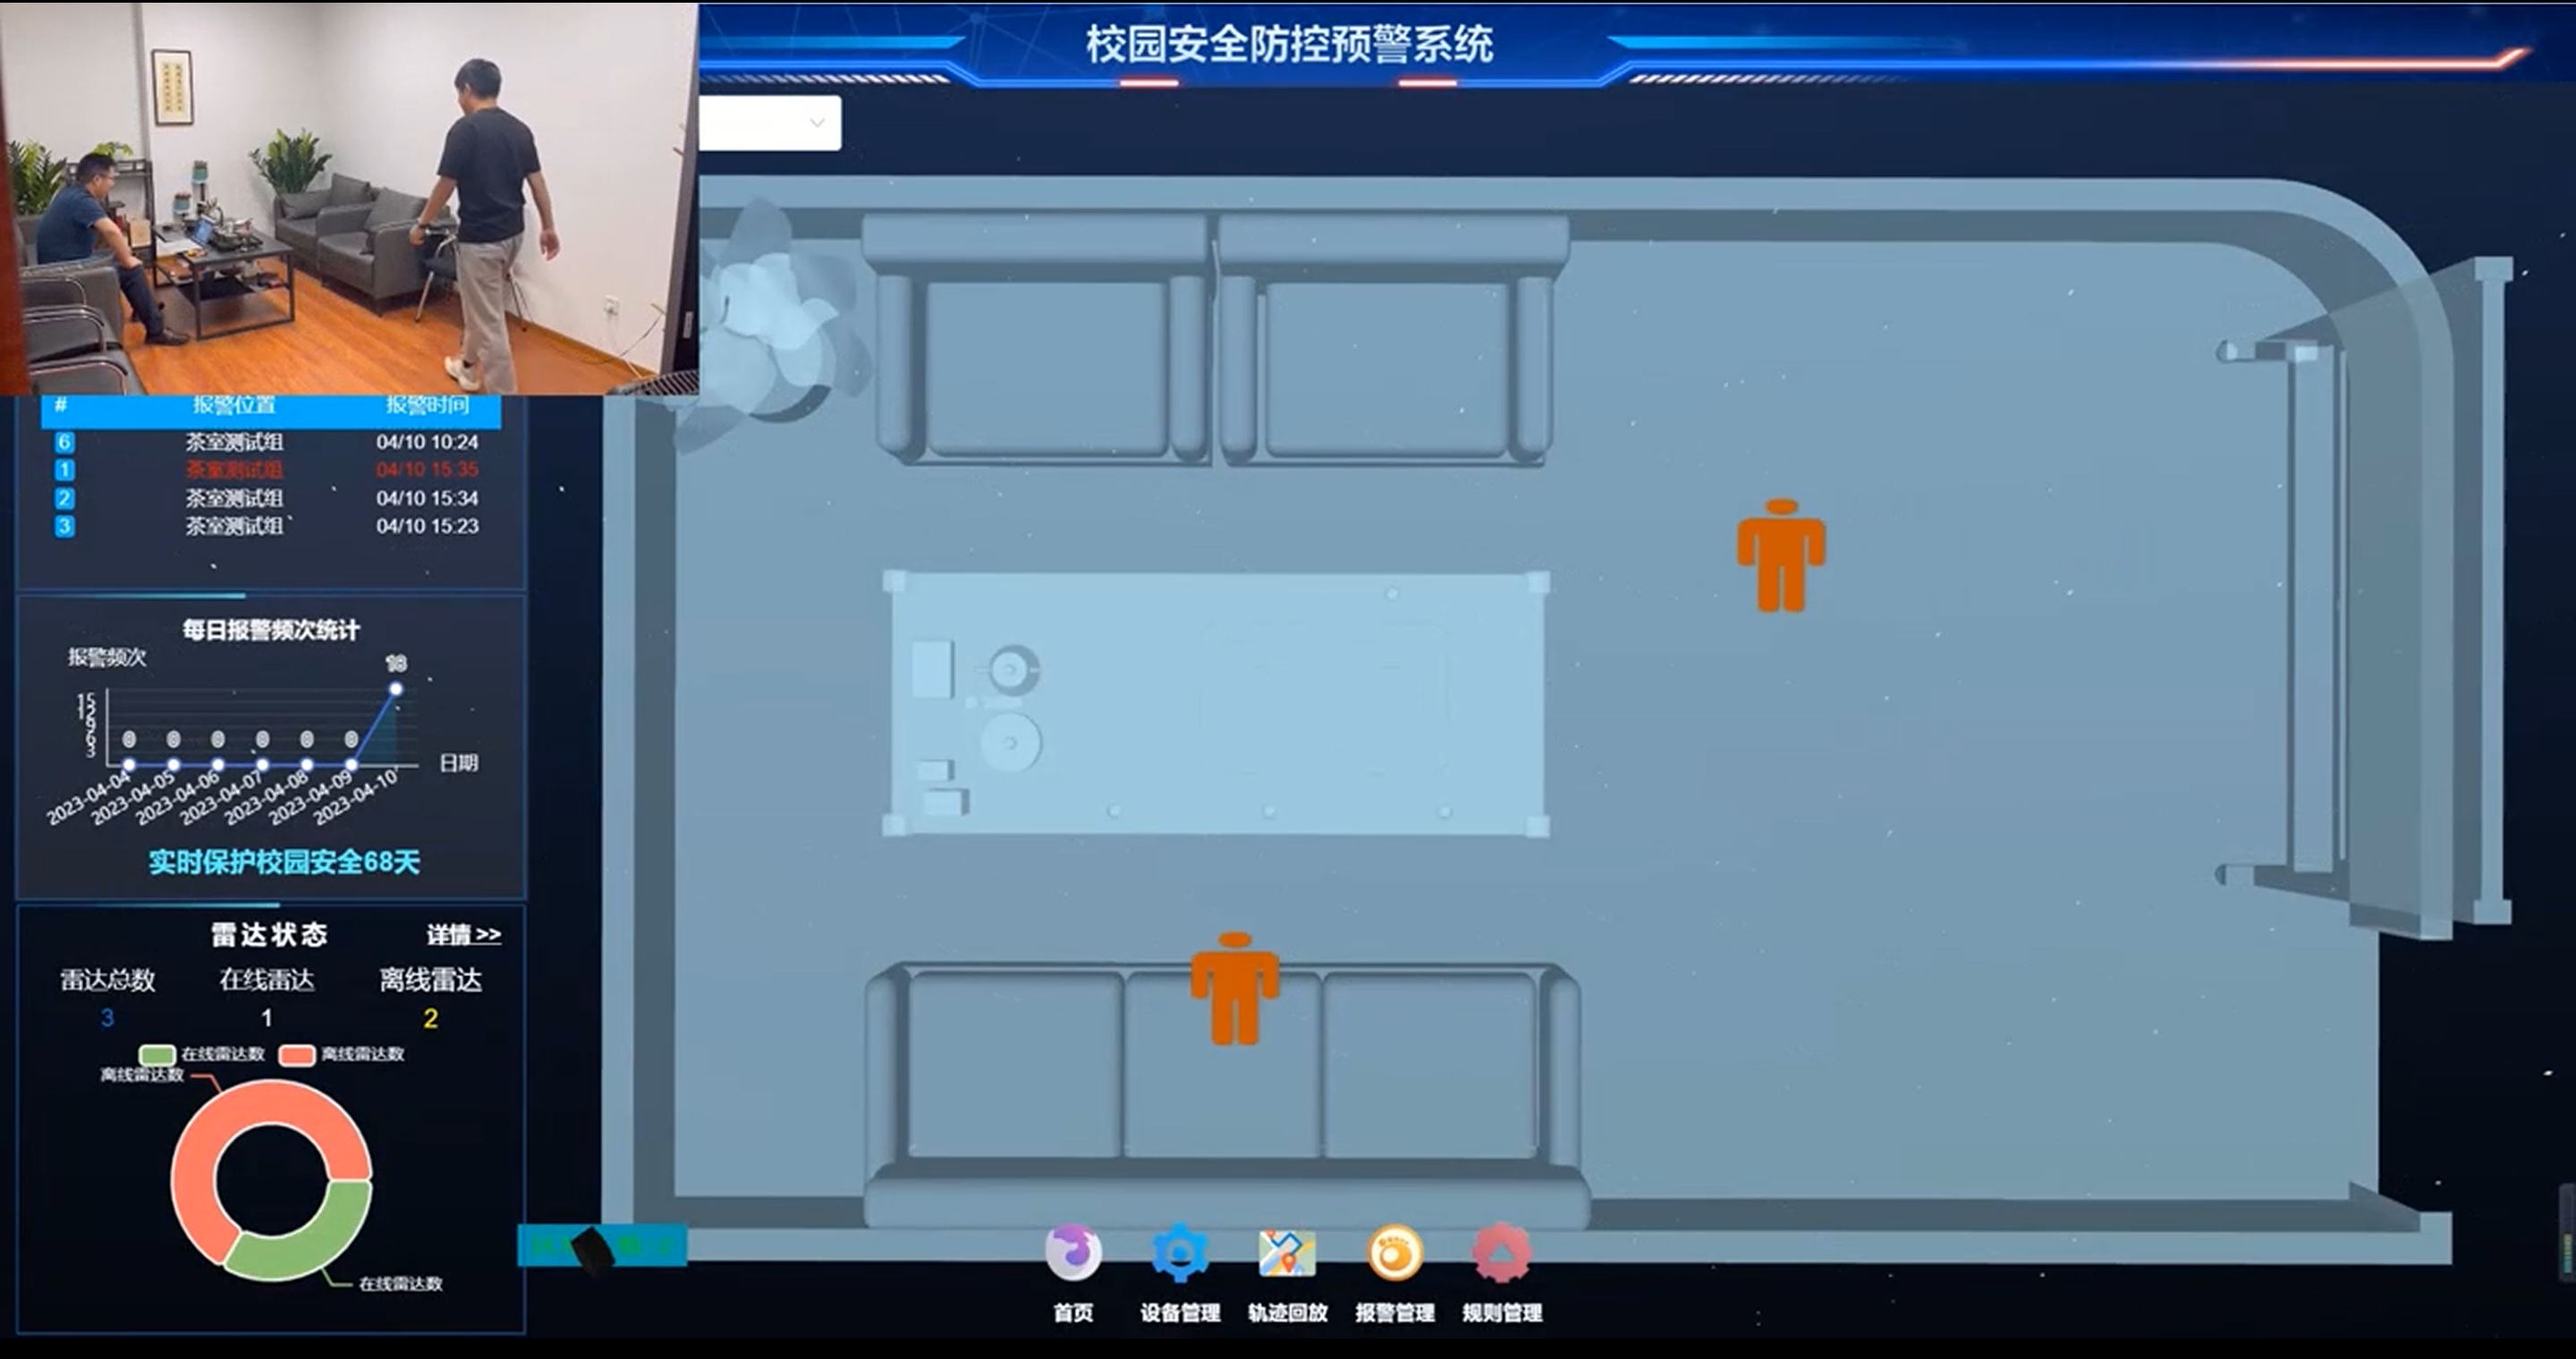
\includegraphics[width = 0.45\linewidth]{images/目标检测.png}}
    \subcaptionbox{目标历史轨迹 \label{目标历史轨迹}}{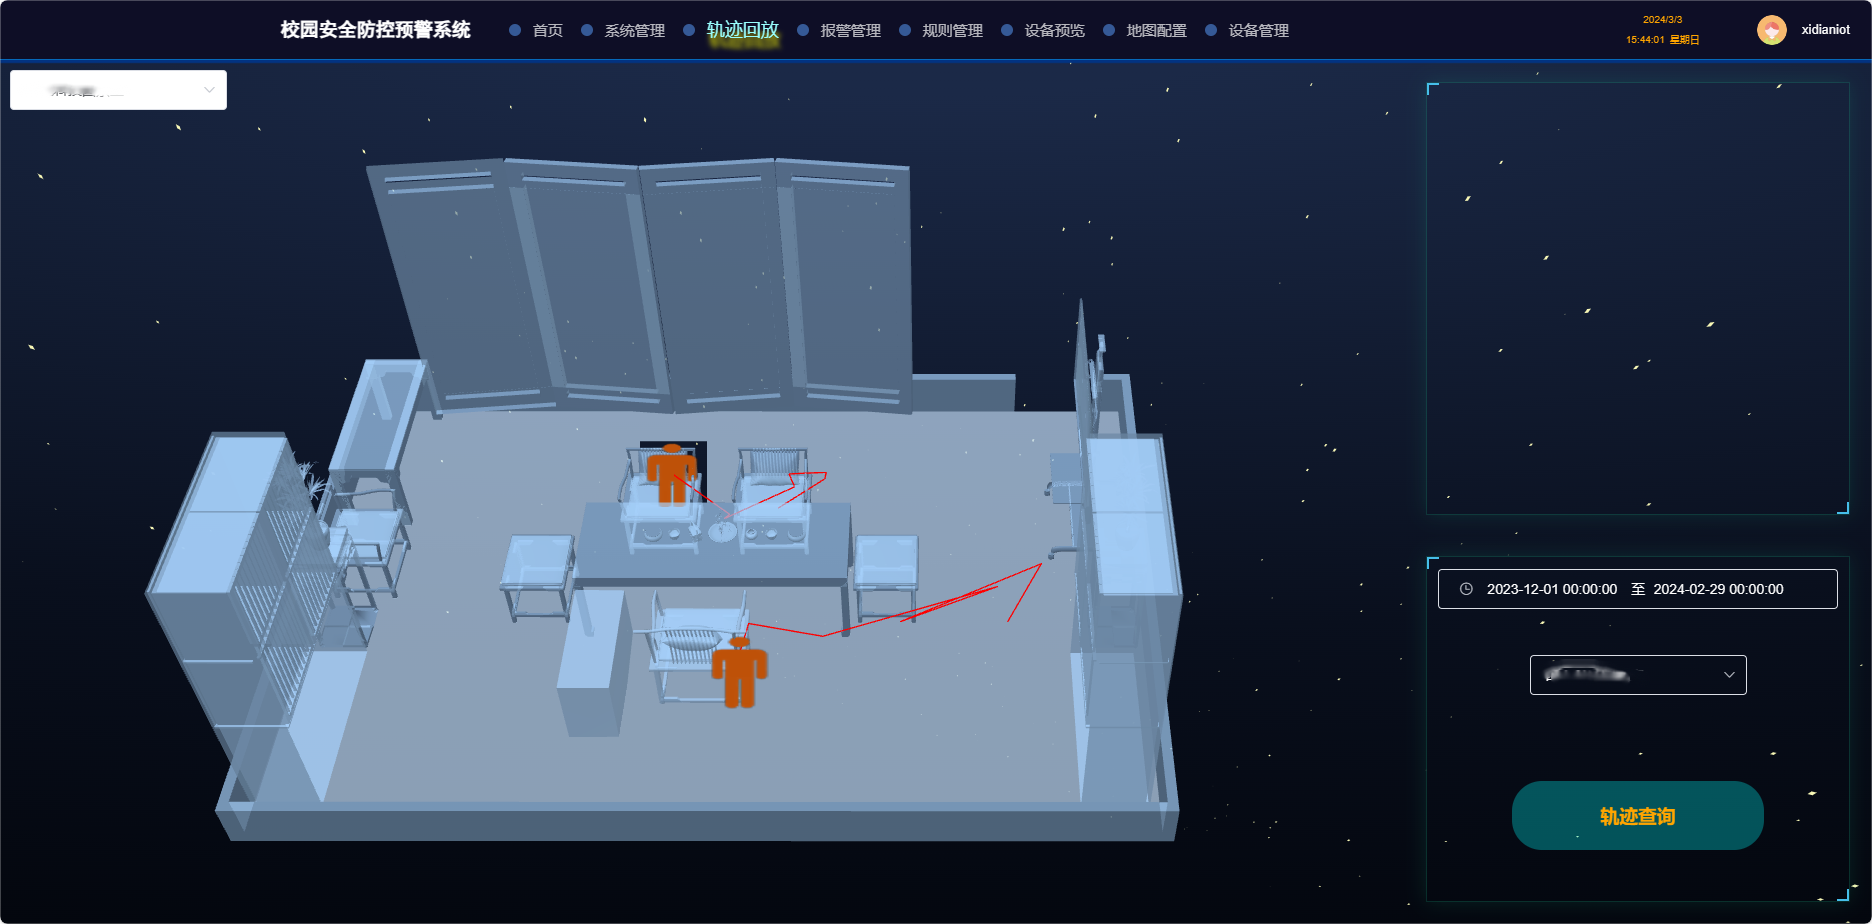
\includegraphics[width = 0.48\linewidth]{images/轨迹回放.png}}
    \caption{目标检测和跟踪功能}
    \label{fig:目标检测和跟踪功能}    
\end{figure}
\par

\subsection{系统性能测试}
\par
(1)点云提取与配准效率测试
\par
毫米波雷达工作时,平均每秒会发送7帧数据,需要对每帧数据提取出点云并根据选的点云进行配准。由于目标追踪的实时性要求,需要及时消费发往消息队列的数据,因此需要对点云提取与配准的效率进行测试。通过脚本向消息队列发送数据,模拟雷达数量增加的负载情况,点云配准模块的配准速率,检测提取与配准的效率。如图\ref{fig:效率测试}所示,随着雷达数量的增加点云提取与配准的响应时间在增加,但是仍在0.01秒以下,效率仍然能够满足实时性的要求。

\begin{figure}[htbp]
    \centering
    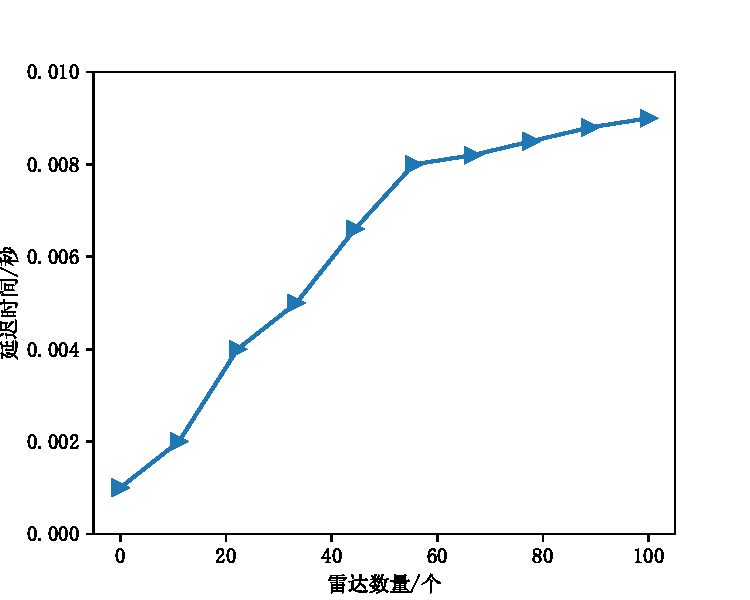
\includegraphics[width = 0.6\linewidth]{figures/效率测试.pdf}
    \caption{效率测试}
    \label{fig:效率测试}    
\end{figure}

(2)配准后点云目标识别准确度测试
\par
为了验证配准后点云的目标识别效果,采集了2个雷达运行1小时的数据,共75600条,其中有目标的数据为15138条,对这些配准后的点云数据进行目标识别,目标识别结果分类如图\ref{目标识别结果分类}所示,统计结果如表\ref{目标识别统计}所示。配准后的点云数据的目标检测准确率达到了96.43\%,精确率达到了92.26\%,召回率达到了96.92\%,说明配准后的点云数据的目标识别效果较好。

\begin{table}[htbp]
    \centering
    \tabcolsep=5mm
    \caption{目标识别结果分类}
    \begin{tabular}{ccc}
        \toprule
        \diagbox{真实}{预测} & 有目标 & 无目标 \\
        \midrule
        有目标 & 14673 & 465 \\
        无目标 & 1231 &  58231 \\
        \bottomrule
    \end{tabular}
    \label{目标识别结果分类}
\end{table}

\begin{table}[htbp]
    \centering
    \tabcolsep=1cm
    \caption{目标识别统计}
    \begin{tabular}{cc}
        \toprule
        评估指标 & 评估值 \\
        \midrule
        有目标数量 & 15138 \\
        无目标数量 & 60462 \\
        准确率 & 96.43\% \\
        精确率 & 92.26\% \\
        召回率 & 96.92\% \\
        \bottomrule
    \end{tabular}
    \label{目标识别统计}
\end{table}
\section{本章小结}
本章主要介绍了基于本文第三章和第四章提出的毫米波雷达目标点检测方案和毫米波雷达点云配准方案构建的一个完整的毫米波雷达点云配准原型系统,并将该系统接入到本课题组研发的校园安防系统中,用于多毫米波雷达场景的毫米波雷达点云数据融合,并且用融合后的数据进行目标检测和跟踪。本章从系统整体设计、系统实现、系统测试三个方面介绍原型系统的设计和实现,验证了毫米波雷达点云检测与配准方案的可行性。

